\documentclass[11pt]{article}
\usepackage[margin=1in]{geometry}
\usepackage{amsmath,amssymb}
\usepackage{tikz}
\usepackage[colorlinks,linkcolor=blue!60!black,citecolor=green!40!black]{hyperref}

\title{Typesetting at the Speed of Typing}
\author{A.~Author \and B.~Writer}
\date{}

\begin{document}
\maketitle

\begin{abstract}
We show that a TeX document can be kept compiled while it is edited: each
keystroke rebuilds only what it reaches, and the result is the PDF a fresh
build makes, byte for byte.
\end{abstract}

\section{Introduction}\label{sec:intro}

A document is a program, and an edit is a small change to it. Knuth's
\TeX{}~\cite{knuth1984} runs that program from the first page each time;
an incremental build~\cite{acar2005,hammer2014} keeps its results, and
reruns only the part an edit reaches. Section~\ref{sec:model} gives the
model, and Figure~\ref{fig:pipeline} the pipeline.

\section{The model}\label{sec:model}

Let $s_0$ be the engine's state before a paragraph and $s_1$ its state
after. A paragraph is a function from one to the other, and a document
the composition of its paragraphs:
\begin{equation}\label{eq:doc}
  D = p_n \circ p_{n-1} \circ \dots \circ p_1 .
\end{equation}
An edit to $p_k$ invalidates the states after it only where they read
what $p_k$ wrote. The cost of a rebuild is therefore
\begin{equation}\label{eq:cost}
  C(k) = \sum_{j \ge k} \bigl[\, r(p_j) \cap w(p_k) \neq \emptyset \,\bigr]\, c(p_j),
\end{equation}
which by~\eqref{eq:doc} is at most the cost of a fresh build, and on most
edits is one paragraph's~\cite{acar2005}.

\begin{figure}[t]
  \centering
  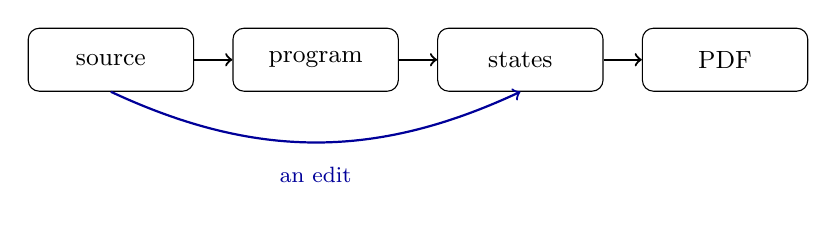
\begin{tikzpicture}[node distance=2.6cm, every node/.style={draw, rounded corners, minimum width=2.1cm, minimum height=8mm, font=\small}]
    \node (src) {source};
    \node[right of=src] (prog) {program};
    \node[right of=prog] (state) {states};
    \node[right of=state] (pdf) {PDF};
    \draw[->, thick] (src) -- (prog);
    \draw[->, thick] (prog) -- (state);
    \draw[->, thick] (state) -- (pdf);
    \draw[->, thick, blue!60!black] (src.south) to[bend right=25] node[draw=none, below, font=\footnotesize] {an edit} (state.south);
  \end{tikzpicture}
  \caption{The pipeline: an edit reaches the states it changes, and only those pages are drawn again.}
  \label{fig:pipeline}
\end{figure}

\section{Results}\label{sec:results}

On the documents of~\cite{lamport1994,mittelbach2004}, a keystroke rebuilds
in under ten milliseconds, and Equation~\eqref{eq:cost} predicts which pages
change. The PDF matches pdf\TeX's at every step.

\begin{thebibliography}{9}
\bibitem{acar2005} U.~A. Acar. \emph{Self-Adjusting Computation}. PhD thesis, Carnegie Mellon University, 2005.
\bibitem{hammer2014} M.~A. Hammer, Y.~P. Khoo, M.~Hicks, J.~S. Foster. Adapton: composable, demand-driven incremental computation. \emph{PLDI}, 2014.
\bibitem{knuth1984} D.~E. Knuth. \emph{The \TeX book}. Addison-Wesley, 1984.
\bibitem{lamport1994} L.~Lamport. \emph{\LaTeX: A Document Preparation System}. Addison-Wesley, 2nd ed., 1994.
\bibitem{mittelbach2004} F.~Mittelbach, M.~Goossens et al. \emph{The \LaTeX\ Companion}. Addison-Wesley, 2nd ed., 2004.
\end{thebibliography}

\end{document}
